
\subsection{Prototype}
\label{sec:prototype}

Un concepto clave es el de \code{prototype}. Este es el mecanismo por naturaleza para "`vincular objetos"' y delegar comportamiento. Comprender lo presentado aquí, resultará de extrema ayuda al momento de analizar la herencia en JavaScript. 

Recordemos que en JavaScript las funciones son objetos, y que los objetos son una colección de propiedades. Al momento de declarar una función, se hace una ligadura de un identificador con el valor de un objeto que es instancia de \code{Function}. Dicho objeto tiene una propiedad especial llamada \code{prototype}, la cual es una referencia a otro objeto, inicialmente vacío. Análogamente, dicho objeto tiene una propiedad llamada \code{constructor} que hace referencia al objeto función que creó la instancia.

\begin{lstlisting}[title={Analizando el \code{prototype} de una función}]
function Foo() {}

console.log(Foo.prototype); // {}

// agregamos propiedades al prototipo
Foo.prototype.valor = 42;
Foo.prototype.bar = function() {
  console.log("bar");
};

console.log(Foo.prototype); // { valor: 42, bar: [Function] }

console.log(Foo.prototype.constructor); // [Function: Foo]

\end{lstlisting}

Podemos hacernos una imagen visual sobre las vinculaciones que hay en memoria al momento de la ejecución mediante el siguiente diagrama:

\begin{figure}[!htbp]
\centering
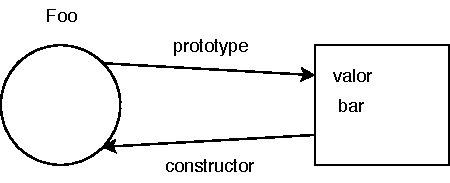
\includegraphics{Figures/Prototype}
\decoRule
\caption[\code{Foo}]{Diagrama del código y los objetos creados.}
\label{fig:prototype}
\end{figure}

Ahora que se mencionó éste concepto, tiene sentido revelar que el constructor de clase \code{Object} no es otra cosa más que una función, y sus métodos \code{toString}, \code{valueOf}, ó \code{hasOwnProperty} forman parte de su "`prototipo"'. Dicho esto, supongamos el siguiente código:

\begin{lstlisting}
var a = new Object();

console.log(a.toString());
\end{lstlisting}

La instancia \code{a} también tiene una propiedad del prototipo. Pero en este caso, en vez de ser \code{prototype}, la misma se llama \code{\_\_proto\_\_}. Una definición vaga sería que las funciones están vinculadas a un prototipo mediante su propiedad \code{prototype} mientras que las instancias se vinculan a su prototipo mediante la propiedad \code{\_\_proto\_\_}. La forma "`genérica"' definida en el estándar de ECMAScript cuando se habla del prototipo, es mediante el término \code{[[Prototype]]}.

Ahora, ?`qué sucede exactamente al momento de hacer \code{a.toString()}? En realidad lo que sucede es que se busca por la propiedad \code{toString} dentro de la instancia de \code{a}, pero al no encontrarse, se seguirá buscando en su \code{[[Prototype]]} (y en caso de no encontrarse, seguiría recursivamente hasta llegar a \code{null}). Ésto es lo que se denomina la cadena del prototipo ("`prototype chain"').

\begin{figure}[H]
\centering
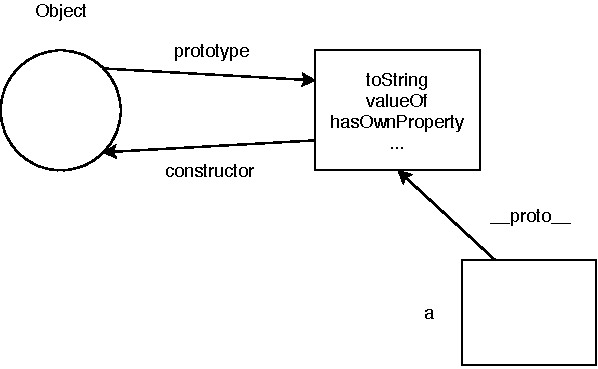
\includegraphics{Figures/Prototype2}
\decoRule
\caption[\code{Object}]{Diagrama del código y la instancia de \code{a}.}
\label{fig:prototype2}
\end{figure}

Sobre el uso del \code{prototype} se hablará con más detalle de esto en las secciones \ref{clases} y \ref{herencia}, donde en ésta última se hará mención a su rol en la herencia prototipada.